With the help of the VsCode's built in profiler we can form a rough idea of what parts of the code
are taking the longest. Here is the output:
\begin{figure}[H]
    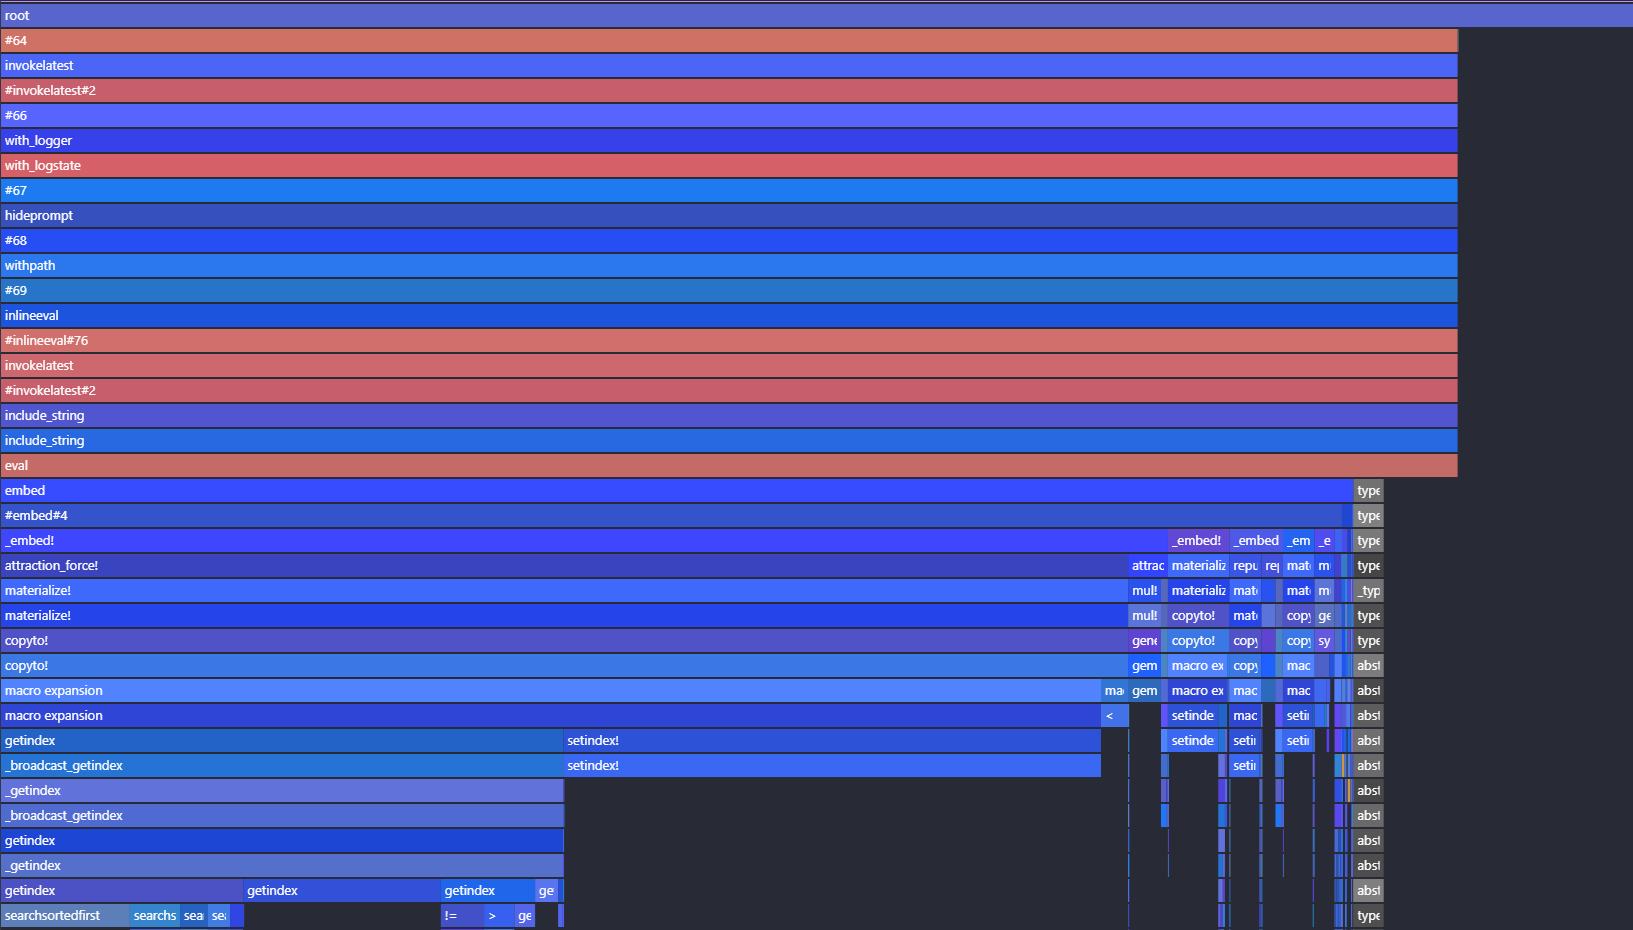
\includegraphics[width=0.5\textwidth]{media/embedProfiling.png}
    \caption{Profiling with attraction\_force!}
\end{figure}
with a profiling time of 132 seconds. \\

After taking a closer look we notice the following resource intensive parts:
\begin{itemize}
    % inclusive time: time spent in the function and all functions it calls
    % exclusive time: time spent in the function itself
    \item function embed, exclusive $\mid$ 20\% or inclusive $\mid$ 83\% 
    \item In embed: 
    \begin{minted}[breaklines,escapeinside=||,
                mathescape=true, 
                linenos, 
                numbersep=3pt, 
                gobble=2, 
                frame=lines, 
                fontsize=\small, 
                framesep=2mm]{julia}
        z = _embed!() # exclusive|19\% or inclusive|82\%
    \end{minted}

    \item In \_embed!(): 
    \begin{minted}[breaklines,escapeinside=||,
                mathescape=true, 
                linenos, 
                numbersep=3pt, 
                gobble=2, 
                frame=lines, 
                fontsize=\small, 
                framesep=2mm]{julia}
        attraction_force!() # exclusive|15\% or inclusive|72\%
    \end{minted}

    \item In attraction\_force!(): 
    \begin{minted}[breaklines,escapeinside=||,
                mathescape=true, 
                linenos, 
                numbersep=3pt, 
                gobble=2, 
                frame=lines, 
                fontsize=\small, 
                framesep=2mm]{julia}
        PQ .= P .* Q; # exclusive|15% or inclusive|69%
    \end{minted}
\end{itemize}

Since we are using a sparse matrix P we can substitute attraction\_force!() with attraction\_force\_symm!().
This is the main change we will be making to the existing embed function to improve its performance. This
version works for symmetric P matrices, and allows multiple threads to be used. Here we can see the 
new results:
\begin{figure}[H]
    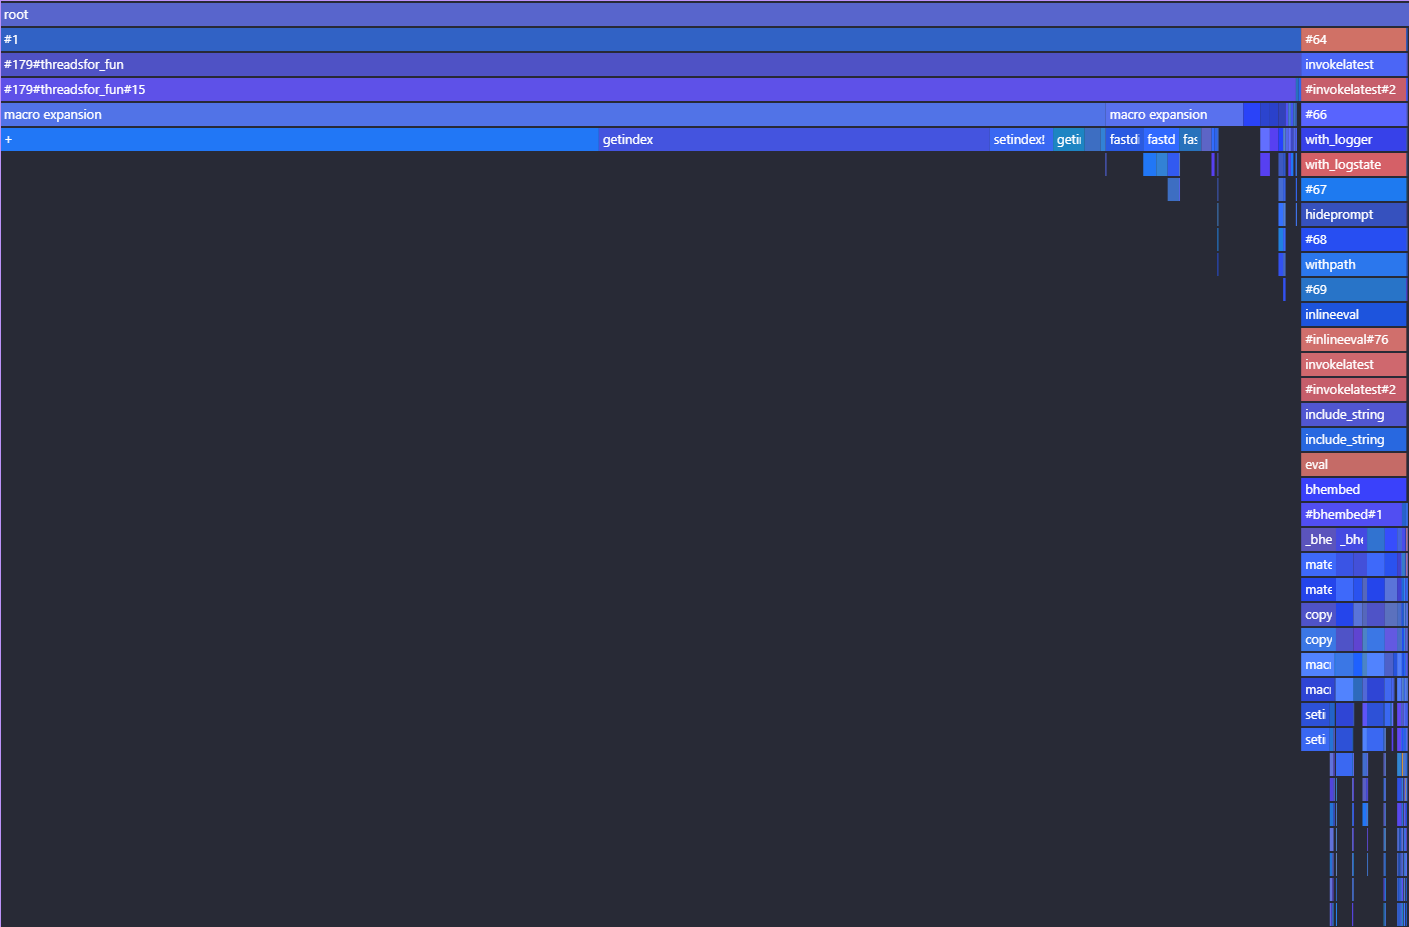
\includegraphics[width=0.5\textwidth]{media/embedProfilingSymm.png}
    \caption{Profiling with attraction\_force\_symm!}
\end{figure}
with a profiling time of 201 seconds. \\

Here the resource intensive parts are:
\begin{itemize}
    \item In attraction\_force!(): 
\end{itemize}
\begin{minted}[breaklines,escapeinside=||,
            mathescape=true, 
            linenos, 
            numbersep=3pt, 
            gobble=2, 
            frame=lines, 
            fontsize=\small, 
            framesep=2mm]{julia}
    Fattr[j,l] += pq * (Yj[l] - Yi[l]) # 78%
\end{minted}

This change introduced a longer profiling time but limited the dependency of the function's speed
to one function which allows us to tweak that one part of the code to improve the overall performance.
It is important to note here that we have not yet set the number of threads for the second version
so the immediately negative results are not indicative of the method's performance. We will later
see exactly how the parameter JULIA\_NUM\_THREADS affects the performance of the function.

% To do: Implement Barnes Hut Algorithm 
% Note that we will be using the "Sparse (without allocations) Barnes-Hut Embeddings" Algorithm.